\subsection*{Model ISO/OSI}
Počítačové sítě vyvíjelo více firem, zpočátku to byly uzavřené a nekompatibilní systémy. Hlavním účelem sítí je však vzájemné propojování, a tak vyvstala potřeba stanovit pravidla pro přenos dat v sítích a mezi nimi. \textbf{Mezinárodní ústav pro normalizaci ISO} (International Standards Organization) vypracoval tzv. referenční model \textbf{OSI (Open Systems Interconnection)}, který rozdělil práci v síti do \textbf{7 vzájemně spolupracujících vrstev}.
\\\\
Jak již bylo řečeno, model ISO/OSI rozděluje síťovou práci na vrstvy. Princip spočívá v tom, že vyšší vrstva převezme úkol od podřízené vrstvy, zpracuje jej a předá vrstvě nadřízené. Vertikální spolupráce mezi vrstvami (nadřízená s podřízenou) je \textbf{věcí výrobce} sítě. Model \textbf{ISO/OSI doporučuje}, jak mají vrstvy \textbf{spolupracovat horizontálně} – dvě stejné vrstvy modelu mezi různými sítěmi (či síťové prvky různých výrobců) musejí spolupracovat. Model je důležitý především pro výrobce síťových komponent. V praktické práci se sítí jej moc nevyužijeme. Umožňuje však pochopit principy práce síťových prvků a zároveň patří k základní terminologii sítí.

\begin{itemize}
\item\textbf{Aplikační vrstva }- Je \textbf{určitou aplikací} (např. oknem v programu) zpřístupňující uživatelům síťové služby. Nabízí a zajišťuje přístup k souborům (na jiných počítačích), vzdálený přístup k tiskárnám, správu sítě, elektronické zprávy (včetně e-mailu)…
\item\textbf{Prezentační vrstva} - Má na starosti \textbf{konverzi dat}, přenášená data mohou totiž být v různých sítích různě kódována. Tato vrstva zajišťuje sjednocení formy vzájemně přenášených údajů. Dále data komprimuje, případně šifruje… V praxi často splývá s relační vrstvou.
\item \textbf{Relační vrstva} - \textbf{Navazuje} a po skončení přenosu \textbf{ukončuje} \textbf{spojení}. Může provádět \textbf{ověřování} uživatelů, \textbf{zabezpečení} přístupu k zařízením…
\item\textbf{Transportní vrstva} - Tato vrstva\textbf{ zajišťuje přenos dat mezi koncovými uzly}. Jejím účelem je poskytnout takovou kvalitu přenosu, jakou požadují vyšší vrstvy. Vrstva nabízí spojově (TCP) a nespojově orientované (UDP) protokoly. (Platí pouze pro \textbf{TCP/IP})
\item\textbf{Síťová vrstva }- Je zodpovědná za spojení a \textbf{směrování mezi dvěma počítači nebo celými sítěmi} (tj. uzly), mezi nimiž neexistuje přímé spojení. Stará se o síťové adresování.
\item \textbf{Linková (spojová) vrstva }- Poskytuje \textbf{spojení mezi dvěma sousedními systémy}. \textbf{Uspořádává data} z fyzické vrstvy do logických celků známých jako \textbf{rámce} (frames). Seřazuje přenášené rámce, stará se o nastavení parametrů přenosu linky, oznamuje neopravitelné chyby. Formátuje fyzické rámce, opatřuje je fyzickou adresou a poskytuje synchronizaci pro fyzickou vrstvu.
\item\textbf{Fyzická vrstva }- Fyzická vrstva definuje všechny elektrické a fyzikální vlastnosti zařízení. Jakým signálem je reprezentována logická jednička, jak přijímací stanice rozezná začátek bitu, jaký je tvar konektoru, k čemu je který vodič v kabelu použit.
\end{itemize}


Rodina protokolů TCP/IP (Transmission Control Protocol/Internet Protocol) obsahuje \textbf{sadu protokolů} pro komunikaci v počítačové síti a je hlavním protokolem celosvětové sítě \textbf{Internet}. Komunikační protokol je množina pravidel, která určují syntaxi a význam jednotlivých zpráv při komunikaci. Architektura TCP/IP je členěna do čtyř vrstev (na rozdíl od referenčního modelu OSI se sedmi vrstvami):

\begin{enumerate}
	\item \textbf{Vrstva síťového rozhraní} (Network interface)
	\item \textbf{Síťová (IP) vrstva} (Internet layer)
	\item \textbf{Transportní vrstva} (Transport layer)
	\item \textbf{Aplikační vrstva }(Application layer)
\end{enumerate}

\noindent\makebox[\textwidth]{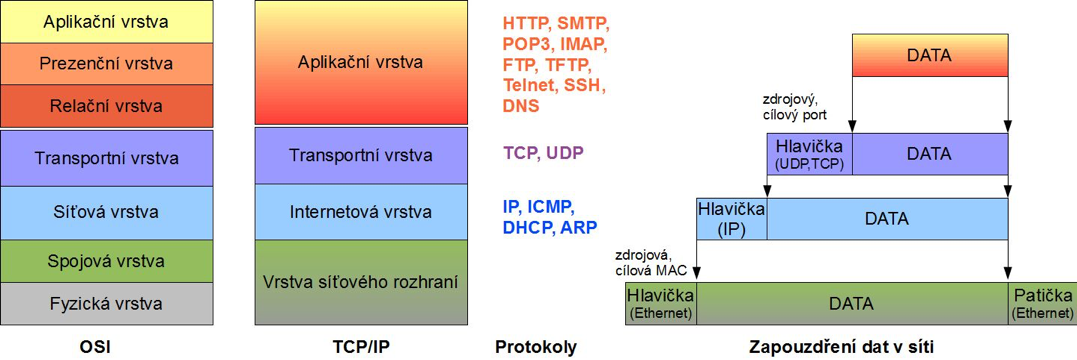
\includegraphics[width=8cm]{assets/4_tcpip}}

Komunikace mezi \textbf{stejnými vrstvami dvou různých systémů} je řízena \textbf{komunikačním protokolem} za použití spojení vytvořeného sousední nižší vrstvou. Architektura umožňuje výměnu protokolů jedné vrstvy bez dopadu na ostatní. Příkladem může být možnost komunikace po různých médiích fyzické vrstvy modelu OSI - ethernet (optické vlákno, kroucená dvojlinka, Wi-Fi), sériová linka.


\subsubsection*{1. Vrstva síťového rozhraní}
Nejnižší vrstva umožňuje \textbf{přístup k fyzickému přenosovému médiu}. Je specifická pro každou síť v závislosti na její implementaci. Příklady sítí: Ethernet, Token ring, FDDI, 100BaseVG, X.25, SMDS.

\subsubsection*{2. Síťová vrstva}
Vrstva zajišťuje p\textbf{ředevším síťovou adresaci}, \textbf{směrování} a předávání datagramů (\textbf{packety}). Protokoly: \textbf{IP}, \textbf{ARP}, \textbf{RARP}, \textbf{ICMP}, \textbf{IGMP}, \textbf{IGRP}, \textbf{IPSEC}. Je implementována ve všech prvcích sítě - směrovačích i koncových zařízeních.

\textbf{Protokol IP (Internet Protocol)}. Od nadřazených protokolů transportní vrstvy obdrží datové segmenty s požadavkem na odeslání. K segmentům připojí vlastní hlavičku a vytvoří IP datagram. V IP hlavičce je především IP adresa příjemce a odesílatele. IP protokol je \textbf{nespojový} (před zahájením výměny dat nevytváří relaci) a \textbf{nespolehlivý} (předání paketů na místo určení není kontrolováno). Paket IP se tedy může ztratit, být doručen mimo pořadí, zdvojen nebo zpožděn. Protokol IP neobsahuje prostředky pro zotavení z chyb tohoto typu. To vše má zajistit nadřízená transportní vrstva – protokol \textbf{TCP}.

\subsubsection*{3. Transportní vrstva}
Transportní vrstva je implementována až v \textbf{koncových zařízeních} (počítačích) a umožňuje proto přizpůsobit chování sítě potřebám aplikace. Poskytuje transportní služby kontrolovaným spojením spolehlivým protokolem \textbf{TCP} (transmission control protocol) nebo nekontrolovaným spojením nespolehlivým protokolem \textbf{UDP} (user datagram protocol).
\\\\
\textbf{Protokol TCP (Transmission Control Protocol)} vytváří \textbf{virtuální okruh} mezi koncovými aplikacemi, zajišťuje tedy spolehlivý přenos dat.
\begin{itemize}
	\item Spolehlivá transportní služba, doručí adresátovi všechna data \textbf{bez ztráty} a ve \textbf{správném pořadí}.
	\item Služba se spojením, má fáze navázání spojení, přenos dat a ukončení spojení.
	\item Transparentní přenos libovolných dat.
	\item \textbf{Plně duplexní spojení}, současný obousměrný přenos dat.
	\item Rozlišování aplikací pomocí portů.
	\item 3-way handshake
	\item Komunikace je řízená pomocí příznakových bitů (ACK, SYN, atd.)
\end{itemize}
\noindent\makebox[\textwidth]{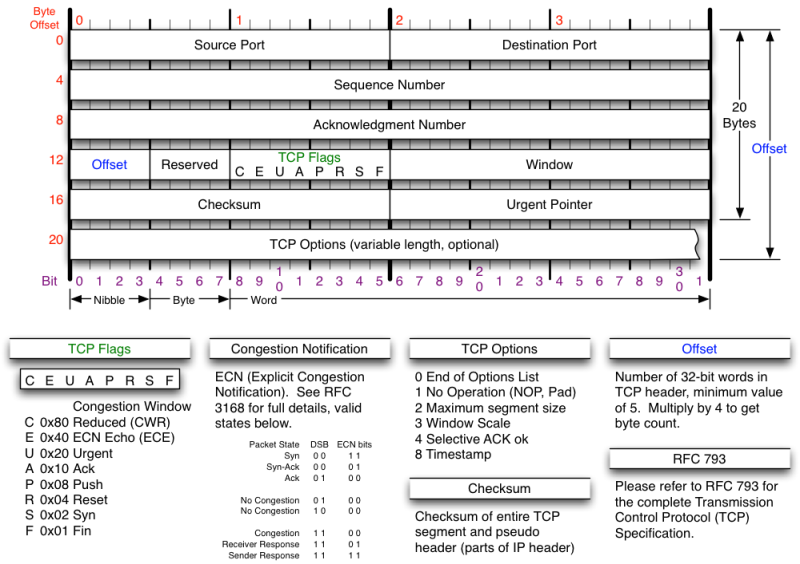
\includegraphics[width=14cm]{assets/4_tcp}}

\textbf{Protokol UDP (User Datagram Protocol)} poskytuje \textbf{nespolehlivou} transportní službu pro takové aplikace, které nepotřebují spolehlivost, jakou má protokol TCP. Nemá fázi navazování a ukončení spojení a už první segment UDP obsahuje aplikační data. UDP je používán aplikacemi jako je \textbf{DHCP}, \textbf{TFTP}, \textbf{SNMP}, \textbf{DNS} a \textbf{BOOTP}.
\begin{itemize}
	\item Nespolehlivá transportní služba, neověřuje zda data došla v pořádku nebo ve správném pořadí.
	\item Nižší režie než u TCP (rychlejší).
	\item Zajištění spolehlivosti je na aplikacích vyšší vrstvy.
	\item Nemá fázi navázání a ukončení spojení, rovnou zasílá data.
	\item Hlavička UDP má pouze 4 části (délku, zdrojový/cílový port, checksum)
\end{itemize}

\noindent\makebox[\textwidth]{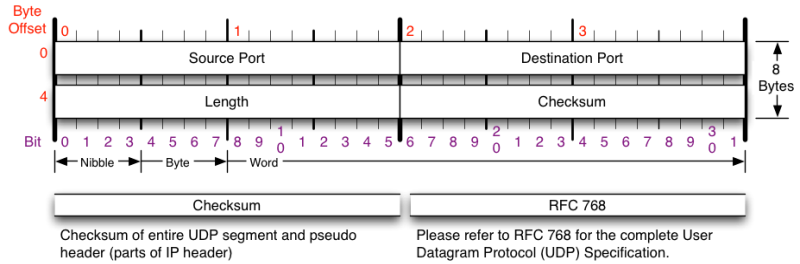
\includegraphics[width=14cm]{assets/4_udp}}

\subsubsection*{4. Aplikační vrstva}
Jedná se přímo o programy (procesy), které využívají přenosu dat po síti ke konkrétním službám pro uživatele. Příklady: \textbf{Telnet} (TCP 23), \textbf{FTP} (TCP 20, 21), \textbf{HTTP} (TCP 80), \textbf{DHCP} (UDP 67, 68), \textbf{DNS} (TCP/UDP 53), \textbf{SSH} (TCP 22).
\\\\
Aplikační protokoly používají vždy jednu ze dvou základních služeb transportní vrstvy: \textbf{TCP} nebo \textbf{UDP}, případně obě dvě (např. DNS). Pro rozlišení aplikačních protokolů se používají tzv. \textbf{porty}, což jsou domluvená číselná označení aplikací. Každé síťové spojení aplikace je jednoznačně určeno \textbf{číslem portu} a \textbf{transportním protokolem} (a samozřejmě adresou počítače).

\subsection*{Překlad síťových adres NAT}
\textbf{NAT (Network address translation)} se většinou používá pro přístup více počítačů z \textbf{lokální sítě} na \textbf{Internet} pod \textbf{jedinou veřejnou adresou}. Překládá zdrojovou a cílovou IP adresu, je realizován na \textbf{routerech}, \textbf{firewallech} většinou zařízeních 3 vrstvy. Umožňuje připojit více počítačů na jednu veřejnou IP adresu - řeší se tak nedostatek přidělených veřejných IP adres. Využívá se překladové tabulky. 
\\\\
\textbf{Výhody:} 
\begin{itemize}
	\item Zvyšuje bezpečnost počítačů připojených za NATem (potenciální útočník nezná opravdovou IP adresu). 
	\item Umožňuje připojit více počítačů na jednu veřejnou IP adresu, čímž se obchází nedostatek IPv4 adres
\end{itemize}
\textbf{Nevýhody:}
\begin{itemize}
	\item Zařízení za NATem nemají skutečné připojení k Internetu (není možné se snadno připojit na zařízení za NATem.)
	\item NAT znemožňuje správnou funkcionalitu některých software
\end{itemize}

\subsubsection*{Typy NATu}
Typicky se využívá kombinace obou níže zmíněných řešení.
\begin{itemize}
	\item \textbf{Statický NAT} - Překladová tabulka je konfigurována manuálně administrátorem.
	\item \textbf{Dynamický NAT} - Obsah překladové tabulky je vytvářen dynamicky v závislosti na síťovém provozu. Veřejné adresy sou alokovány jednotlivým spojením jejich vypůjčením z \textbf{NAT Poolu}.
	\item \textbf{Network adress and por translation NAPT} - Několik uzlů využívá pouze jednu veřejnou IP adresu. Jednotlivé uzly jsou identifikovány pomocí různých čísel portů.
\end{itemize}

\subsection*{IPv6}
IPv6 \textbf{nahrazuje} dosluhující protokol IPv4. Přináší zejména \textbf{masivní rozšíření adresního prostoru} a zdokonalení schopnosti přenášet \textbf{vysokorychlostně data}. Starší protokol IPv4 poskytuje omezený adresní prostor – teoreticky $2^32$ adres. IPv6. Obsahuje celkem $2^128$ adres. Většina přenosových a aplikačních vrstev protokolů vyžaduje malé nebo žádné změny pro funkčnost s IPv6. Výjimkami jsou protokoly aplikací zahrnující adresy síťové vrstvy např.: FTP. \textbf{Multicast} je součástí základní specifikace IPv6 na rozdíl od IPv4, kde byl zaveden později. IPv6 nepoužívá \textbf{broadcast} na místní linku. Každá adresa má \textbf{128b}. \textbf{Odstraněna potřeba NAT}. Protokol pro IP vrstvu šifrování a autentizaci \textbf{IPsec} je integrální součástí souboru protokolů IPv6, na rozdíl od IPv4, kde je přítomen volitelně (obvykle ale implementován).
\\\\
IPv6 adresy se obvykle zapisují jako osm skupin čtyř hexadecimálních číslic: \textbf{2001:0db8::1428:57ab}. Vzhledem k zdlouhavému zápisu se může nejdelší sekvence nul nahradit \textbf{::}. 4 nuly můžeme nahradit jednou.

\subsubsection*{IPv6 Packet}
Paket IPv6 se skládá ze dvou hlavních částí: hlavičky a těla.
\begin{itemize}
	\item \textbf{Verzi} - 4 bity, verze 6
	\item \textbf{Dopravní třídu} - 8 bitů na prioritu paketu. Úroveň priority se dělí na rozsahy: kde zdroj podporuje kontrolu přetížení a bez podpory kontroly přetížení.
	\item \textbf{Pojmenování toku} - 20 bitů pro správu QoS. Původně určeno pro speciální obsluhu aplikací reálného času, nyní se nepoužívá.
	\item \textbf{Délka těla} - 16 bitů pro délku těla paketu. Při vynulování se nastaví „jumbo“ tělo (skok za skokem)
	\item \textbf{Následující hlavička} - 8 bitů, určuje další vnořený protokol. Hodnoty se shodují s hodnotami definovanými pro IPv4.
	\item \textbf{Zdrojová a cílová adresa} - 128 bitů na každou adresu.
	\item\textbf{Hop limit }- 8 bitů, číselně definuje počet povolených přechodů síťovými prvky. Každý přechod znamená snížení čísla o 1.
\end{itemize}

\noindent\makebox[\textwidth]{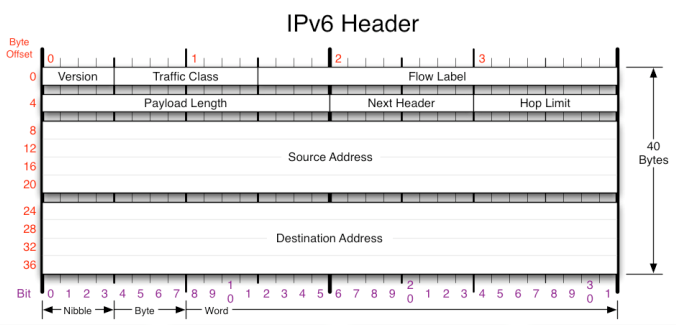
\includegraphics[width=16cm]{assets/4_ipv6}}
